mechanisms should work for amazon/lvl/samsung


Environment and Integrity Checks, wenn die umgebung falsch ist, kann die app verändert werden. deswegen von vornherein ausschließen, dass die bedingungen dafür gegeben sind.\cite{munteanLicense}

in order to remove/disable lvl they have to modify the code
unless done precisely can be detected by code (signature muss geändert werden von lucky um dex fiel gültig zu halten)\cite{developersSecuring}

\begin{figure}[h]
    \centering
    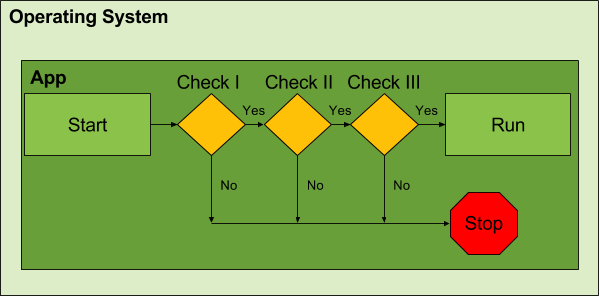
\includegraphics[width=0.8\textwidth]{data/verificationNowAdditional.png}
    \caption{Introduction of additional tests to check environment and integrity of the application}
    \label{fig:verificationNowAdditional}
\end{figure}
his does not stop luckypatcher in anyway but it stops the app from working in case the environment is not suitable
force close im falle von falschem outcome, entspricht nicht android qualität
\url{http://developer.android.com/distribute/essentials/quality/core.html} aber so wird es dem user klarer dass seine application gecracked ist. harmlosere variante dialog anzeigen oder element nicht laden.

all tampering counter measurements have kind of the same pattern, boolean check, simple method == simple fix, can be nulled easily when code is known, just as easy to crack as LVL when you know the code, but attackr has to invest some time to understand code and to build counter measurement, in addition with Section~\ref{subsection:counter-improve-obfuscation} this can get annoying, evtl create native versions because harder to crack
even though it is simple it adds a little bit extra work to attack and when cobined this grows exponential
automatischen angriff aushebenln indem andere unbekannte tests die erst entdeckt werden müssen
add additional test, have to be cracked as well, first attacker has to realize them and find them
all tampering counter measurements have kind of the same pattern, boolean check, simple method == simple fix, can be nulled easily when code is known, just as easy to crack as LVL when you know the code, but attackr has to invest some time to understand code and to build counter measurement, in addition with Section~\ref{subsection:counter-improve-obfuscation} this can get annoying, evtl create native versions because harder to crack
even though it is simple it adds a little bit extra work to attack and when cobined this grows exponential

es gibt verschieden punkte um die integrity der application sicherzustellen. dies beinhaltet die umgebung debugg oder rootzugriff, die suche nach feindliche installierte applicationen oder checks nach der rechtmäßigen installation und rechtmäßigen code.
